\chapter{Solving Strategies}
\label{chap:strategies}

This chapter describes and compares different strategies and approaches used and tested during solver development.


%%%%%%%%%%%%%%%%%%%%%%%%%%%%%%%%%%%%%%%%%%%%%%%%%%%%%%%%%%%%%%%%%%%%%%%%%%%%%%%%%%
\section{Phases of problem solving}

In section ~\ref{sec:mathForm} the complete linear program used as basic foundation for solving the problem was introduced. From practice, though, arose the need of split the problem into some phases.

The first partition is related to virtual teaching resources. Since virtual professors should be used only when there is no real professor available, it makes sense to consider virtual resources apart from the initial problem, that is, first to solve a model with only real resources and then solving a second model that allows virtual resources only for those demands not satisfied at first stage. The only obstacle to such partition is whether gaps in student's timetable are directly prohibit by the model (see constraints ~\ref{constrStudentGap}). In this scenario, by partitioning the problem, any case of non-satisfied demand with a real professor will generate an empty time slot at an extremity of a day, but never between allocated classes. The problem is that this could easily prevent satisfaction of other demands when professor availability is restricted, which is very common. 

As a simple example, suppose that due to a lack of teaching resource a demand of some class for Mathematics lessons will inevitably be non-satisfied with a real professor. The History professor, Norah Jones, can only teach at 08:00 on Monday morning. If lessons have one-hour duration, and if due to professors limited availability no other course can be assigned at 9:00 am on Monday, but only later, then either an one-hour gap will be generated from 9:00 to 10:00 am and later filled in by a Math lesson with a virtual resource, or Prof. Jones will be prevented for teaching to the History lesson to the class, so that a gap is not created. In case of students' gaps constraints are being considered, necessarily only the second option would last, which is actually not interesting, since a History demand would be not satisfied due to inconsistency of input data for Mathematics teaching resource. This small example gives us a glimpse of how important is input data consistency and how aspects not obviously related at first sight are actually connected.

Thus, splitting the problem into real and virtual resources phases is advised only when students' gaps constraints have not been included in the linear program. Fortunately, if student's available timetable fits exactly his courses demands, there is no need of such constraints!


%%%%%%%
\subsection{Real teaching resource}

As was indicated while introducing the concept of professor at section ~\ref{defprof}, professors might have different importance levels, which means that a professor can have his assignments prioritized over others. Such distinction emerged from practice, when analyzing some possible solutions to the timetabling problem of a Brazilian school. What happens is that, as discussed in section ~\ref{sec:accuracy}, actual timetabling for educational institutions is a political just as much as a scheduling problem. It might be acceptable if the timetable of a fresh professor of the school does not end up as compact as it would be desired, but it is unacceptable that timetable of an old professor of the school, considered as a loyal employee, does not respect a minimum and high quality level.

Real teaching resources should then receive different treatment depending on their priorities.

\paragraph{First Priority}

We consider, as the first phase of the problem solving process, the solving of a linear program containing only real and first priority professors. This avoids that particularities and restrictions on lower-priority professors interfere with higher-priority professors assignments.

\paragraph{Second Priority}

In the second phase of the problem solving process we solve a linear program containing only real professors, with all priority levels, but ensuring timetable quality for first priority professors reached at solution of the first phase.


%%%%%%%
\subsection{Virtual teaching resource}

After solving the problem using all real resources available, if there is any non-satisfied demand, it is time to consider virtual teaching resources. The best solution found with real resources at previous phase is fixed and virtual professors are used only to satisfy the remaining demands, filling in empty time slots in students timetables.


%%%%%
\myparagraph{Maximizing remaining demand satisfaction through the best use of virtual resources}

Supposing that the best solution found until this moment has been fixed and thus prevented from being modified, then the last thing to do is to satisfy the maximum of remaining demands with virtual resources. 

Since virtual teaching resources have neither quality nor overlapping constraints, they are very easy assignments and could even be done as a post-processing. Still, we chose to make use of mathematical programming to do it, for 2 reasons: first, the model formulation and implementation is just the same one we have been using, except that current real solution must be fixed and virtual resources allowed; second, we can take advantage of mathematical programming to easily remove some symmetry around virtual resources usage.

It is very common for professors to restrict their available teaching time. Suppose the Biology professor, Glen Hansard, is only available on Tuesdays and Fridays, and the Geography professor, Freddie Mercury, is only available on Wednesdays and Fridays. Due to the global lack of teaching resources, a virtual professor must be assigned to the Biology and Geography lessons of class $C1$. For purposes of simplification, consider that both Biology and Geography courses have 1 credit each. Class $C1$'s timetable must have at least 2 empty time slots then, otherwise its demand would be greater than it can support. Finally, suppose that assignments of other courses attended by $C1$ could be rearranged so that we have the following possibilities:
\begin{itemize}
\item an empty time slot on Monday and on Wednesday, or
\item an empty time slot on Tuesday and on Wednesday.
\end{itemize}

Now, the decision to be made is to which time slot assign the Biology and the Geography virtual lessons. Are they equally good? Possible solutions are:
\begin{enumerate}
\item assign Biology to Monday and Geography to Wednesday, or \label{bmgw}
\item assign Biology to Tuesday and Geography to Wednesday, or \label{btgw}
\item assign Geography to Monday and Biology to Wednesday. \label{gmbw}
\item assign Geography to Tuesday and Biology to Wednesday, or \label{gtbw}
\end{enumerate}

The difference is that, in case of a meeting with virtual teaching resource, assigning the course lesson to a time slot at which no capable professor has registered availability implies either hiring a new professor for teaching the course or negotiating with the current capable professors their availabilities. On the other hand, assigning the course lesson to a time slot at which a capable professor has registered availability necessarily implies hiring a new professor, since if a capable professor is already registered at that time slot and still the lesson is being taught by a virtual resource, it means either that the professor was assigned to another class at that moment or that he has been blocked by some quality constraint.

Bearing this in mind, best options for virtual assignment in the previous example are ~\ref{gmbw} and ~\ref{gtbw}, because neither Prof. Hansard is available on Wednesday nor Prof. Mercury is available on Monday and Tuesday, the intermediate option is ~\ref{bmgw}, and the worst option is ~\ref{btgw}, since days chosen for courses classes are exactly the days respectively already available for both professors.

\paragraph{Objective function for virtual resource phase}

To simplify notation, we define $KV_{d}$ as being a set containing all variables $k$ of virtual professor for course $d$. Such set can be split into two subsets according to professors availabilities, let us say $KVPA_{d}$ and its complement $\overline{KVPA}_{d}$, so that $KVPA_{d} \cup \overline{KVPA}_{d} = KV_d$, where $KVPA_{d}$ is the subset of all variables $k$ of virtual professor for course $d$ and for a time slot at which some real capable professor has registered availability.

Then, what we aim is to satisfy the remaining demand using virtual teaching resources, while giving preference to those assignments that reduce the certainty of having to hire new professors and guaranteeing the current solution. Since virtual resource phase is much simpler and we do not have conflicting goals, an unified objective function works just fine and is enough. This last goal is achieved by:

\begin{align*}
   \mbox{g = MIN  }
		(\sum\limits_{a \in A}\sum\limits_{d \in D} fd_{d,a}
		+		
		0.00001 \cdot \sum\limits_{k \in KVPA_{d}} k_{pv,i,d,u,t,h})
		\\
		\mbox{\textit{subjected to assignments made in the best}}
		\\
		\mbox{\textit{solution found when considering real resources}}
\end{align*}




%%%%%%%%%%%%%%%%%%%%%%%%%%%%%%%%%%%%%%%%%%%%%%%%%%%%%%%%%%%%%%%%%%%%%%%%%%%%%%%%%%
\section{Goal programming}

Just as in any other kind of problem, the feasibility of a linear model for a timetabling problem depends utterly on input data set. In general, there is no guarantee that all demanded requirements can be satisfied with the specified available resources, even because usually there are several and conflicting objectives. Therefore, specially in a commercial solver, it is important to treat some idealistic hard constraints as highest priority soft constraints, otherwise the solver could frequently generate an infeasible model.

In real life it is useless for an educational institution to have a solution that satisfies all demands of students for courses, but which does not respect some important quality requirements. Bearing this in mind, in addition to the feasibility issue, the model presented at this work, unlike most authors, does not consider demand satisfaction as a hard constraint. Essential quality requirements are modeled as hard constraints though, and demand satisfaction is treated as the highest priority objective, followed by some further goals.

A \textbf{multi-objective function} unifies disparate goals of the model in a single weighted sum of preferences. Such approach, although simpler, depends on very subjective choice of weights and is not always consistently reliable, specially if involving trade-off, when objectives are mutually conflicting. It can be very difficult to quantify quality.

An alternative approach is using a priority line for the different goals. According to the institution preferences, one optimizes the problem in a sequence of steps, where each step is responsible for a goal, from the most to the least important. For each step a different and specific objective function is used and the feasible solution space is subject to features of the best solution found at the previous step. Such approach is known as \textbf{preemptive goal programming} and is following detailed.


%%%%%%%%%%%%%%%%%%%%%%%%%%%%%%%%%%%%%
\subsection{General concept}

A goal programming model seeks to simultaneously take into account several objectives or goals that are concern to a decision maker. While a linear programming model consists of constraints and a single objective function to be maximized or minimized, a goal programming model consists of constraints and a set of goals that are prioritized in some sense.
In both linear and goal programming problems, if the constraints are inconsistent, there are no feasible solutions for the model. In goal programming, however, one can expect that although there is a set of feasible solutions satisfying the constraints, none of them may simultaneously satisfy all the conflicting goals of the organization. The objective of goal programming is to find a solution that satisfies the true constraints and comes closest to meeting the stated goals.

In \textbf{lexicographic} or \textbf{preemptive goal programming} the decision maker orders the unwanted deviations into a number of priority levels, with the minimization of a deviation in a higher priority level being infinitely more important than any deviations in lower priority levels. A lexicographic goal program can be solved as a series of linear programs and should be used when there is a clear priority ordering amongst the goals to be achieved. The idea behind the preemptive goal programming approach is that lower priority level goals should not be attained at the expense of higher priority goals --- they are preempted.

If the decision maker is more interested in direct comparisons of the objectives then weighted or \textbf{nonpreemptive goal programming} should be used. In this case all the unwanted deviations are multiplied by weights, reflecting their relative importance, and added together as a single sum to form the achievement function, which converts the goal programming model into a linear programming model.

G\"{u}enalay and Sahin use goal programming at \cite{Guenalay2006} to satisfy instructors' preferences as much as possible.


%%%%%%%%%%%%%%%%%%%%%%%%%%%%%%%%%%%%%
\subsection{Applying Goal Programming}

Next are presented the possible goal programming approaches for a real resource phase of the problem.


%%%%%%%%%%%%%%
\subsubsection{Preemptive Goal Programming}

Following are listed the goals, ordered by priority, considered at this work for real resource phase when using preemptive goal programming. For each step there is a specific objective function and the respective feasible solution space is additionally constrained by the solution of the previous phase. We draw attention to the ease of changing priorities order and adding or removing goals; and to the nonexistence of coefficients multiplying variables at each objective function.

\begin{enumerate}

%%%%%
\item{Maximizing demand satisfied by real professors}

\begin{align*}
   \mbox{g1 = MIN  } \sum\limits_{a \in A}\sum\limits_{d \in D} fd_{d,a}
\end{align*}

%%%%%
\item{Minimizing the number of lessons, in case of courses that can have classes merged}

\begin{align*}
  \mbox{g2 = MIN  } \sum\limits_{i \in I_{d}} \sum\limits_{d \in Dm} z_{i,d}
	\\
	\sum\limits_{a \in A}\sum\limits_{d \in D} fd_{d,a} \le g1
\end{align*}

Where the additional constraint restricts the search-space to solutions where the satisfied demand is no less than the value $g1$ achieved at previous step.

%%%%%
\item{Minimizing real professor displacement}

\begin{align*}
  \mbox{g3 = MIN  } \sum\limits_{p \in P} \sum\limits_{t \in T} \sum\limits_{u1 \in U} \sum\limits_{u2 \in U} Time_{u1,u2} \cdot desloc_{p,t,u1,u2}
	\\
	\sum\limits_{a \in A}\sum\limits_{d \in D} fd_{d,a} \le g1
	\\
	\sum\limits_{i \in I_{d}} \sum\limits_{d \in Dm} z_{i,d} \le g2
\end{align*}

Where the additional constraint restricts the number of sharable classes to be no more than the minimal value $g2$ achieved at previous step.

%%%%%
\item{Minimizing gaps in real professor's timetable}

\begin{align*}
   \mbox{g4 = MIN  } \sum\limits_{p \in P} \sum\limits_{t \in T} \sum\limits_{f \in F} fpgap_{p,t,f}
	\\
	\sum\limits_{a \in A}\sum\limits_{d \in D} fd_{d,a} \le g1
	\\
	\sum\limits_{i \in I_{d}} \sum\limits_{d \in Dm} z_{i,d} \le g2
	\\
	\sum\limits_{p \in P} \sum\limits_{t \in T} \sum\limits_{u1 \in U} \sum\limits_{u2 \in U} Time_{u1,u2} \cdot desloc_{p,t,u1,u2} \le g3
\end{align*}

Where the additional constraint restricts the solution space to the minimum real professor displacement achieved at previous step.

%%%%%
\item{Minimizing number of days and sessions of day used in real professor's timetable}

\begin{align*}
   \mbox{g5 = MIN  } \sum\limits_{p \in P} \sum\limits_{t \in T} ( pt_{p,t} + \sum\limits_{f \in F} ptf_{p,t,f})
	\\
	\sum\limits_{a \in A}\sum\limits_{d \in D} fd_{d,a} \le g1
	\\
	\sum\limits_{i \in I_{d}} \sum\limits_{d \in Dm} z_{i,d} \le g2
	\\
	\sum\limits_{p \in P} \sum\limits_{t \in T} \sum\limits_{u1 \in U} \sum\limits_{u2 \in U} Time_{u1,u2} \cdot desloc_{p,t,u1,u2} \le g3
	\\
	\sum\limits_{p \in P} \sum\limits_{t \in T} \sum\limits_{f \in F} fpgap_{p,t,f} \le g4
\end{align*}

Where the additional constraint restricts the solution space to the minimum amount of gaps in real professors' timetable achieved at previous step.

\end{enumerate}


The final solution for the real resource phase is the one with cost equal to $g5$, achieved at last stage. If an optimal solution is achieved for all steps, then at the end of the last step we guarantee that the final solution found is the best one with respect to the order of priorities.

\begin{figure}[H]
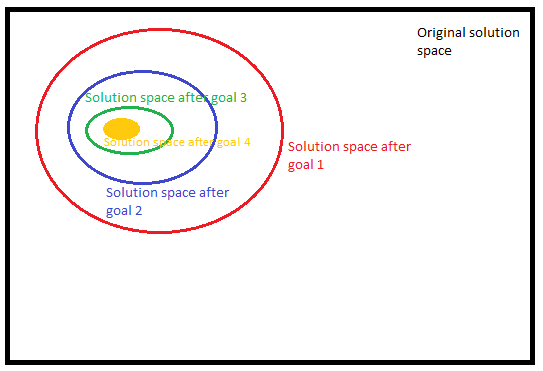
\includegraphics[scale=0.6]{figures/goalProgSpace.png}
\centering
\caption{Solution spaces are limited and encapsulated after each goal optimization step.}
\end{figure}

\fixme{atualizar etapas na figura}




%%%%%%%%%%%%%%
\subsubsection{Nonpreemptive Goal Programming}
\fixme{or Multi-objective function? no final nao tem mta diferenca!}

Following there is the unified objective function considered at this work for the real resource phase. Although here it is even easier than at goal programming to change priorities order and adding or removing goals, there is the necessity of choosing coefficients for variables at objective function.

$$
\begin{array}{rl}
   \mbox{MIN} &
			\lambda \cdot \sum\limits_{a \in A}\sum\limits_{d \in D} \cdot fd_{d,a}
      \\
      &
      + \epsilon \cdot \sum\limits_{p \in P} \sum\limits_{t \in T} \sum\limits_{f \in F} fpgap_{p,t,f}
      \\
      &
			+ \sigma \cdot \sum\limits_{p \in P} \sum\limits_{t \in T} \sum\limits_{u1 \in U} \sum\limits_{u2 \in U} Time_{u1,u2} \cdot desloc_{p,t,u1,u2}
			\\
			&
      + \theta \cdot \sum\limits_{i \in I_{d}} \sum\limits_{d \in Dm} z_{i,d}
			\\
			&
			+ \alpha \cdot \sum\limits_{p \in P} \sum\limits_{t \in T} ( pt_{p,t} + \sum\limits_{f \in F} ptf_{p,t,f})
\end{array}
$$

An unified objective function is more appropriate when goals have not a strict priority order, in the sense that their combinations can produce solutions that are Pareto efficient.

So, the question when choosing the approach is whether one wants to order or weight goals.


%%%%%%%%%%%%%%%%%%%%%%%%%%%%%%%%%%%%%
\subsection{Comparing results}

Through preemptive goal programming it is easier to understand the best solution found by the optimization process and the reasons of non-satisfaction of different goals, specially when the number of goals to be achieved through the objective function increases.





%%%%%%%%%%%%%%%%%%%%%%%%%%%%%%%%%%%%%%%%%%%%%%%%%%%%%%%%%%%%%%%%%%%%%%%%%%%%%%%%%%%%%%%%%%%%%%%%%%%
%%%%%%%%%%%%%%%%%%%%%%%%%%%%%%%%%%%%%%%%%%%%%%%%%%%%%%%%%%%%%%%%%%%%%%%%%%%%%%%%%%%%%%%%%%%%%%%%%%%
\section{Polishing Method}

For real-world school timetabling, where problem size is not small, solving the hole MIP introduced at section ~\ref{sec:mathForm} of chapter ~\ref{chap:mipformulation} at once with a MIP Solver like Gurobi or Cplex has been shown to be ineffective and unworkable. Tests made with an ordinary size school \fixme{falar o tamanho da escola testada} have shown that generic MIP Solvers find it already very difficult to converge to a good integer solution. For bigger schools, both the linear relaxation and the branch and bound phase are \textit{very} hard and have proven themselves impossible to be solved by current MIP solvers.

An auxiliary method was then developed for helping convergence while solving the MIP. It is described at next sections and referred here as a \q{polishing method}.


%%%%%%%%%%%%%%%%%%%%%%%%%%%%%%%
\subsection{The general idea}

Given a $lp$ model and an initial feasible solution $s$, the idea of a polishing method is iteratively to solve models $lp'$ similar but easier than the original model, such that any feasible solution for $lp'$ is also a feasible solution for $lp$ and the solution at the end of each iteration is always at least as good as at the beginning. In another words, it is generated a sequence of feasible solutions with monotonically (but not strictly) increasing quality.

Suppose that a solution $s \in \mathbb{Z}^n$ is feasible to $lp$. Let us split the set of $n$ integer variables into 2 subsets, such that $n=p+q, p \ge 0, q\ge 0$, $s_p \in \mathbb{Z}^p$, $s_q \in \mathbb{Z}^q$ and thus $s = s_p \cup s_q$. The basic principle is that optimizing a linear program $lp' = lp \cap s_p$ generates a feasible solution $s'$ to $lp'$ which is also feasible to $lp$ and at least as good as $s$. All variables and constraints of the original problem are still present in the new problem, but cuts were added, which limit the solution space based on $s_p$, resulting in a more restricted solution space. The smaller is the solution space, the easier is the solver convergence.

The aim of cutting the solution space here is not to eliminate non-promising search-space regions, but to search in a smaller and treatable space. There is then no guarantee that the actual optimal solution $s*$ for $lp$ is in or out the eliminated region, but it is ensured that the optimal solution $s'*$ for $lp'$ is equal or better than the previously known solution $s$. It is thus not interesting to keep these cuts after solving $lp'$. Instead, the idea is to restore the original problem and add others cuts, now based on the new solution $s'$. Doing that iteratively, we create a guide for the solver.

So, what solution space of $lp'$ looks like? At each polishing iteration, the limitation of the search-space takes place through the tightening of a subset of variables bounds based on the initial solution $s$. Suppose the trivial example where the solution space is equal to the cube $c = [0, 4]^3 \in \mathbb{Z}^3$ and the feasible solution $s \in \mathbb{Z}^3$ is $s = \{s_1=3,s_2=2,s_3=0\}$. A possible limitation based on $s$ would be to tighten the interval bounds of the first dimension to the value of $s_1$, such that the resulting solution space is $c' = [3, 3][0, 4][0, 4]$. Such tightening clearly eliminates one dimension of the search-space and keeps the feasible solution $s$. Consequently, optimizing over $c'$ can not lead to a worse solution, because in the worst-case scenario the best solution is $s$ itself.

Because at the beginning of the polishing process the solution is supposedly a very poor quality one and the search-space is a wide unexplored space, the percentage of variables with tightened bounds starts high (lets say around 90\%) and drops as the limited search-space is potentially exhausted and solution improvement stagnates. If at the end of the polishing this percentage reaches 0\%, then the considered linear program is the original one and its optimization ends the process. If an optimal solution is found at the 0\% stage, then it is surely an optimal solution for the original problem. For too hard linear programs though, it is unlikely that the polishing reaches this last stage, and the process is then interrupted by time limit. Generally speaking, nothing can be said about optimality for a solution found before the 0\% stage.



%%%%%%%%%%%%%%%%%%%%%%%%%%%%%%%%%%%%%
\subsection{The polishing algorithm developed for the problem}

Following a detailed pseudo-algorithm for the polishing method developed for the school timetabling problem is described. The main algorithm, specified at ~\ref{alg:polishing}, contains the general steps of the polishing process.

The essential requirements for using the polishing method are a linear program and a feasible initial solution. In addition, in case a proved optimal solution is not achieved, run time limits are used as stopping criteria: a total maximum execution time for the method ($maxTime$), and a maximum execution time since the last solution improvement occurrence ($maxTimeNoImprov$).

The algorithm starts at line ~\ref{polish:ln:init} with some initialization, defined at ~\ref{alg:init}. The current solution $sol$ is set with the initial solution, the percentage $perc$ of variables with fixed bounds is initialized with 90\%, the MIP optimization time limit $timeIter$ is initialized with 70 seconds, all blocks are set free and, in the case of several blocks which share teaching resources, blocks may be clustered to assist further bounds tightening. The polishing process begins at line ~\ref{polish:ln:iter}, where at each iteration a new optimization cycle takes place. Every cycle has 4 main steps: variables bounds tightening (line ~\ref{polish:ln:fix}), optimization of the tightened linear program (line ~\ref{polish:ln:opt}), update of percentage of fixed variables and of time limit for each optimization (line ~\ref{polish:ln:perc}), and variables bounds release (line ~\ref{polish:ln:unfix}). At line ~\ref{polish:ln:runtime} the polishing run time limit is checked. All these steps have their respective algorithms detailed ahead.

\begin{algorithm}[H]
  \caption{Polishing method
    \label{alg:polishing}} 
  \begin{algorithmic}[1]
    \Require{$lp$ model, any initial feasible solution $solIni$, the maximum run time $maxTime$ for the hole polishing method and the maximum run time $maxTimeNoImprov$ of polishing without improvement}
		\Ensure{A final feasible solution $sol$ for the $lp$ model at least as good as the initial solution $solIni$}
    \Statex
    \Function{Polish}{$solIni$, $maxTime$, $maxTimeNoImprov$}		
			\State \textsc{init}$()$																	\label{polish:ln:init}
			\Let{$okIter$}{$true$}
      \While{$okIter$}																					\label{polish:ln:iter}
          \State \textsc{fixVars}$()$														\label{polish:ln:fix}
					\State \textsc{optimize}$()$													\label{polish:ln:opt}
					\State \textsc{updatePercAndTimeIter}$()$							\label{polish:ln:perc}
					\State \textsc{unfixVars}$()$													\label{polish:ln:unfix}
					\State \textsc{checkRunTimeLimit}$()$									\label{polish:ln:runtime}
      \EndWhile
     \State \Return{$sol$}
    \EndFunction
	\Statex	
  \Algphase{Initialization}
    \Procedure{init}{$lp$, $solIni$}														\label{alg:init}
				\Let{$sol$}{$solIni$}
				\Let{$perc$}{$90$}
				\Let{$timeIter$}{70}
				\State set all blocks free
				\State cluster blocks according to teaching staff sharing
    \EndProcedure
  \end{algorithmic}
\end{algorithm}		
		
% --------------------------------------
Algorithm ~\ref{alg:fixVars} describes the step of tighten variables ranges. Different approaches were tested and those which best succeed are shown below. The main algorithm requires the original linear program, a feasible solution and the percentage of fixation; and ensures a resultant linear program for which a subset of variables have tightened bounds and where the subset size is proportional to the fixation percentage. Three different types of fixation were implemented: fixing all lessons of a subset of blocks (line ~\ref{fixVars:blocks}), fixing lessons of random classes (line ~\ref{fixVars:lessons}) and fixing random assignments of professors to classes (line ~\ref{fixVars:profs}). The procedure for fixation of lessons per block, detailed at line ~\ref{alg:fixBlocks}, requires the set $FB$ of blocks that should be completely fixed at the current iteration, besides a feasible solution for the $lp$. Then, every potential lesson that belongs to a fixed block has the lower and upper bounds of its corresponding variable $x$ tightened according to its value at the current solution $sol[x]$. The procedure for fixation of random classes, detailed at line ~\ref{alg:fixLessons}, requires a percentage value $perc$ that indicates how much of the current solution should be fixed. Such amount of classes is then randomly selected and stored in the set $FC$ (lines ~\ref{alg:fixLessons1}-~\ref{alg:fixLessons2}). Following, analogously to blocks fixation, every lesson variable $x$ for which the class belongs to $FC$ has its lower and upper bounds tightened according to its value at the current solution $sol[x]$ (lines ~\ref{alg:fixLessons3}-~\ref{alg:fixLessons4}). Lastly, the procedure for fixation of random professors assignments, detailed at line ~\ref{alg:fixProfs}, likewise requires the solution fixation percentage, selects the corresponding amount of variables $y$ responsible for assigning professors to classes and tights their bounds.
		
\begin{algorithm}[H]
  \caption{Fixing variables' values
    \label{alg:fixVars}}
  \begin{algorithmic}[1]
    \Require{$lp$ model, a feasible solution $sol$ and the percentage $perc$ of fixation}
		\Ensure{A resultant $lp$ model with a random subset of its variables with fixed bounds and therefore easier to solve}
    \Procedure{fixVars}{}
			\State \textsc{fixBlocks}$()$																\label{fixVars:blocks}
			\State \textsc{fixVarsClassesBounds}$()$										\label{fixVars:lessons}
			\State \textsc{fixVarsProfBounds}$()$												\label{fixVars:profs}
    \EndProcedure
	\Statex	
  \Algphase{Fixing blocks}
    \Require{$lp$ model, a feasible solution $sol$ and a set $FB$ of fixed blocks}
    \Procedure{fixBlocks}{}																				\label{alg:fixBlocks}
			 \For{each variable $x_{u} \in lp$ such that $u \in FB$}
				\Let{$lowerbound_{x}$}{$sol[x]$}
				\Let{$upperbound_{x}$}{$sol[x]$} 
			 \EndFor
    \EndProcedure
	\Statex
  \Algphase{Decide which classes to fix and fix the corresponding lessons bounds}
    \Require{$lp$ model, a feasible solution $sol$ and the percentage $perc$ of fixation}
		\Ensure{A subset of lessons variables with tightened bounds}
    \Procedure{fixVarsClassesBounds}{}															\label{alg:fixLessons}
			\Let{$FC$}{$\emptyset$}
			\For{each variable $z \in lp$}																\label{alg:fixLessons1}
					\If{$rand() \ge perc$}
						\Let{$FC$}{class represented by $z$}										\label{alg:fixLessons2}
					\EndIf
			\EndFor
			\For{each variable $x \in lp$ such that class of $x$ is in $FC$}	\label{alg:fixLessons3}
					\Let{$lowerbound_{x}$}{$sol[x]$}
					\Let{$upperbound_{x}$}{$sol[x]$} 															\label{alg:fixLessons4}
			\EndFor
    \EndProcedure
	\Statex
	\Algphase{Fix bounds of variables of professors}
    \Require{$lp$ model, a feasible solution $sol$ and the percentage $perc$ of fixation}
    \Procedure{fixVarsProfBounds}{}																	\label{alg:fixProfs}
			\For{each variable $y \in lp$}	
					\If{$rand() \ge perc$}
						\Let{$lowerbound_{y}$}{$sol[y]$}
						\Let{$lowerbound_{y}$}{$sol[y]$} 
					\EndIf
			\EndFor
    \EndProcedure	
  \end{algorithmic}	
\end{algorithm}

% --------------------------------------
Algorithm ~\ref{alg:optimize} describes the steps around a request for optimization. It requires a linear program $lp$ and a feasible solution $sol$, and ensures a final updated solution $sol$ at least as good as the initial one. The linear program considered here is the one resulting from the variables bounds tightening step. The procedure sets the time limit $timeIter$ for the optimization, sets $sol$ as an initial solution and optimizes the model using a MIP solver. When optimization ends, run time is recorded at $runtime$ and the extra time, i.e., the difference between time limit and run time, is recorded at $timeLeft$. These values may later be used for updating $timeIter$ with a more appropriate value. Finally, if optimization succeeded, the current solution $sol$ is updated with the new solution and elapsed time since last solution improvement is updated.

\begin{algorithm}[H]
  \caption{Optimize
    \label{alg:optimize}}
  \begin{algorithmic}[1]
    \Require{$lp$ model, a feasible solution $sol$ to $lp$}
		\Ensure{A final updated feasible solution $sol$ for the $lp$ model at least as good as the initial solution}
    \Procedure{optimize}{}
			\State set optimization time limit equal to $timeIter$
			\State set $sol$ as a start solution to $lp$	
			\State optimize $lp$
			\Let{$runtime$}{run time spent at the optimization}
			\Let{$timeLeft$}{\abs{timeIter - runtime}}
			\If{optimization succeeded}
				\Let{$sol$}{new best solution found}
				\If {solution was not improved}
					\State update elapsed time without improvement
				\Else
					\State reset elapsed time without improvement
				\EndIf
			\EndIf
    \EndProcedure	
  \end{algorithmic}	
\end{algorithm}		

% --------------------------------------
Algorithm ~\ref{alg:updatePercAndTimeIter} is responsible for taking actions, whether there is a need, on percentage of solution fixation or on optimization time limit. Such actions are based on the last optimization performance. At line ~\ref{update:allfree} it is checked if the linear program is completely free, i.e., if it is the original $lp$. If so, then the current iteration is the last one and there is nothing last to be updated. Otherwise, actions differ according to whether the $lp$ was solved to guaranteed optimality (line ~\ref{update:smallgap}) or not (line ~\ref{update:biggap}). If a proved optimal solution was found, it suggests that the $lp$ was not hard, and actions may be decrease the portion of the problem that is fixed (line ~\ref{smallgap:percblock}) and adjust optimization time limit (line ~\ref{smallgap:time}). On the other hand, if optimality was not reached, it suggests that the $lp$ may be too hard. Thus, in case of solution has not been improved when compared to the previous iteration (line ~\ref{biggap:noimprove}), efforts to facilitate the problem are made, such as updating the set of fixed blocks (line ~\ref{biggap:nextblock}) and adjusting time limit (line ~\ref{biggap:time}).


\begin{algorithm}[H]
  \caption{Update percentage of fixed variables, fixed blocks and maximum time per iteration
    \label{alg:updatePercAndTimeIter}}
  \begin{algorithmic}[1]
    \Require{$lp$ model}
    \Procedure{updatePercAndTimeIter}{}
			\If{\textsc{allFree}$()$}																						\label{update:allfree}
				\Let{$okIter$}{$false$}
				\Return
			\EndIf
	    \If {\textit{lp was solved until optimal or gap is small enough}}
			  \State \textsc{updatePercAndTimeIterSmallGap}$()$									\label{update:smallgap}
			\Else
				\State \textsc{updatePercAndTimeIterBigGap}$()$										\label{update:biggap}
			\EndIf
    \EndProcedure	
		\Statex
		\Algphase{Update percentage of fixed variables, fixed blocks and maximum time per iteration for small gap case}
			\Procedure{updatePercAndTimeIterSmallGap}{}													\label{alg:smallgap}
				\State \textsc{adjustPercOrBlock}()																\label{smallgap:percblock}
				\State \textsc{adjustTime}()																			\label{smallgap:time}
			\EndProcedure
		\Statex
		\Algphase{Update percentage of fixed variables, fixed blocks and maximum time per iteration for big gap case}
			\Procedure{updatePercAndTimeIterBigGap}{}																	\label{alg:biggap}
				\If{solution was not improved at the current iteration}									\label{biggap:noimprove}
					\Let{$acresm$}{0, if all blocks are currently free; or 10 otherwise}	
					\State \textsc{setNextRandFreeBlocks}$(acresm)$												\label{biggap:nextblock}
					\State \textsc{adjustTime}()																					\label{biggap:time}
				\EndIf
			\EndProcedure			
  \end{algorithmic}	
\end{algorithm}


% --------------------------------------
Algorithm ~\ref{alg:setNextRandFreeBlocks} is a procedure to adjust the set of blocks that will be free or fixed at next iteration. It requires an incremental value $percAdjust$ to the percentage of fixed blocks, which can be negative if the aim is to hamper the problem, null if no change of percentage is aimed, or positive if the aim to facilitate the problem. Such percentage ($percBlockFixed$) is updated at line ~\ref{nextblock:perc}. At line ~\ref{nextblock:enoughit} the number of consecutive iterations with fixed blocks is verified and, if it is sufficient, all blocks are set free for the next iteration. The concept of what is sufficient is subjective, but tests have worked well with a maximum of 4 consecutive iterations. Otherwise, blocks to set free at next iteration are chosen by a routine at line ~\ref{nextblock:choose}. Such routine resets the current set of free blocks, and decides randomly at line ~\ref{choose:setcluster} whether the type of block fixation will be by cluster or not. If so, a cluster of blocks is selected at line ~\ref{choose:cluster} and every block of the cluster is set free. Then, the number of fixed blocks is checked and, while it doesn't reach at least the percentage $percBlockFixed$, blocks are set free randomly.

\begin{algorithm}[H]
  \caption{Set free and fixed blocks for the next iteration
    \label{alg:setNextRandFreeBlocks}}
  \begin{algorithmic}[1]
    \Require{an incremental $percAdjust$ of the fixed blocks percentage}
		\Ensure{an updated set of fixed or free blocks for next iteration}
    \Statex
    \Procedure{setNextRandFreeBlocks}{$percAdjust$}
			\Let{$percBlockFixed$}{$percBlockFixed + percAdjust$} 		\label{nextblock:perc} %\Comment{update percentage of fixed blocks for next iteration}
      \If{there is enough consecutive iterations with fixed blocks}	\label{nextblock:enoughit}
      	\State free all blocks for the next iteration
      	\Return
      \EndIf
      \State \textsc{chooseAndSetFreeBlocks}()												\label{nextblock:choose}
    \EndProcedure
	  \Statex
	  \Algphase{Choose and set free blocks for the next iteration}
    \Procedure{chooseAndSetFreeBlocks}{}
			\State reset set of free blocks
			\Let{useCluster}{true or false, randomly chosen with $50\%$ of chance of true}						\label{choose:setcluster}
			\If{useCluster} 																					%\Comment{type of fixing blocks is per cluster}
				\State choose a cluster of blocks and set it free																				\label{choose:cluster}
			\EndIf
			\While{number of free blocks $<$ $(100-percBlockFixed)\cdot$ \textit{total of blocks}}		\label{choose:free}
			\State choose randomly a block and set it free
			\EndWhile
    \EndProcedure
  \end{algorithmic}
\end{algorithm}

% --------------------------------------
Algorithm ~\ref{alg:adjustTime} adjusts optimization time limit for the next iteration according to the current iteration performance. If the linear program was set completely free for next iteration, which means it is the original problem, then it will be the last optimization, and therefore all remaining time for polishing is set. If solution was not improved and time limit was reached before proving optimality, then it suggests that time limit may be too low and its increasing is proceeded at line ~\ref{time:increase}. Otherwise, if solution was improved, then time limit is checked at line ~\ref{time:decrease}. The increasing of time, described at line ~\ref{alg:increase}, is proportional to the current percentage of fixed variables and blocks. Just as a precaution so that time limit does not increase too much, an upper bound for it may be forced at line ~\ref{increase:max}. The decreasing of time, described at line ~\ref{alg:decrease}, occurs whether the current time limit has been shown to be much higher than necessary, which is measured by comparing the difference between the run time and the time limit ($timeLeft$) and the extra time required for the sake of precaution ($minExcess$).


\begin{algorithm}[H]
  \caption{Adjust time
    \label{alg:adjustTime}}
  \begin{algorithmic}[1]
    \Require{values of performance of the current iteration optimization}
		\Ensure{optimization time limit adjusted for next iteration}
    \Procedure{adjustTime}{}
			\If{\textsc{allFree}$()$}
				\Let{$timeIter$}{$getRemainingTime()$}												\label{time:lastit} %\Comment{next iteration will be the last one}
				\Return
			\EndIf
			\If {solution was not improved at the current iteration \textbf{and} time limit for the iteration was reached}
				\State \textsc{increaseTime}()													\label{time:increase} %\Comment{time limit reached  increases time limit}
			\EndIf
			\If {solution was improved at the current iteration}
				\State \textsc{decreaseTime}()													\label{time:decrease} %\Comment{Adjust time limit in case it is too high}
			\EndIf
    \EndProcedure	
	  \Statex
	  \Algphase{Increase time}
    \Procedure{increaseTime}{}																	\label{alg:increase}
			\Let{$incremTime$}{10}																		%	\Comment{increases the time limit by a fixed amount}
			\Let{$incremTime$}{$incremTime + (100-perc)\cdot 0.2$}		%\Comment{increases the time limit the more perc is close to 0}
			\Let{$incremTime$}{$incremTime + (100-percBlockFixed)\cdot 0.2$}	%\Comment{increases the time limit the more blocks are free}
			\Let{$timeIter$}{$timeIter + incremTime$}
			\If{$timeIter > MaxTimeImposedPerIteration$}							\label{increase:max}
				\Let{$timeIter$}{$MaxTimeImposedPerIteration$} 					%\Comment{possibly forces a reduction of $timeIter$, whether a maximum time per iteration is imposed.}
			\EndIf
    \EndProcedure	
	  \Statex
	  \Algphase{Decrease time}
    \Procedure{decreaseTime}{}																	\label{alg:decrease}
				\Let{$minExcess$}{$max(0.5\cdot timeIter, 50)$}
				\If{$timeLeft > minExcess$} 														\label{decrease:excess} %\Comment{Adjust time limit in case it is too high}
					\Let{$timeIter$}{$runtime+minExcess$}
				\EndIf
    \EndProcedure			
  \end{algorithmic}
\end{algorithm}

% --------------------------------------
Algorithm ~\ref{alg:adjustPercOrBlock} is responsible for adjusting the percentage of solution that is fixed. The decrease of fixed solution amount can take place in 2 situations: either optimality was very fast achieved (line ~\ref{perc:easy}) or optimality was achieved but solution was not improved at all (line ~\ref{perc:decrease}). The first one is not really necessary --- it is basically just an attempt to speed up the method. The second one is essential, because it is the natural way of decreasing fixation, which means getting closer to the actual linear program. The idea is that the search-space size should be enlarged whenever the optimal solution value equals the current best solution value, since it suggests that search-spaces with the current size may have been exhausted or would make small contributions. The subroutine for decreasing solution fixation, called \textsc{decreasePercOrFreeBlock} and described at ~\ref{alg:decreaseperc}, requires a value that might be subtracted of the fixation percentage. It can actually either decide to change and enlarge the set of free blocks (line ~\ref{decreaseperc:anyblock}) or indeed subtract the percentage $perc$ of solution fixation (line ~\ref{decreaseperc:decrease}). The principle is that decreasing the value $perc$ is an \q{one way street}, i.e., we can never backtrack and increase $perc$, while on the other hand the number of fixed blocks can vary according to the difficulty faced when solving $lp$. Thus, the actual decreasing of the value $perc$ takes place only when all blocks are free at the current iteration.


\begin{algorithm}[H]
  \caption{Adjust percentage of fixed variables or fixed blocks
    \label{alg:adjustPercOrBlock}}
  \begin{algorithmic}[1]
		\Require{values of performance of the current iteration optimization}
    \Procedure{adjustPercOrBlock}{}
			\If{$optimal$ \textbf{and} $timeLeft > 0.7\cdot timeIter$} \label{perc:easy} %\Comment{decrease the fixed portion if it was easy (fast) to solve}
				\State \textsc{decreasePercOrFreeBlock}$(5)$	
			\Else 
				\If{$optimal$ \textbf{and} \textbf{not} $improved$}	  	\label{perc:decrease}	%\Comment{decrease the fixed portion if no improvement was made}	
					\State \textsc{decreasePercOrFreeBlock}$(10)$		
				\EndIf	
			\EndIf
    \EndProcedure	
	  \Statex
	  \Algphase{Decrease percentage of fixed variables or free blocks}
		\Require{a value to be subtracted of the fixation percentage}
    \Procedure{decreasePercOrFreeBlock}{$percToSubtract$}				\label{alg:decreaseperc}
			\If{$percToSubtract \le 0$}
				\Return
			\EndIf
			\If{there is any block currently fixed}										\label{decreaseperc:anyblock}
				\State \textsc{setNextRandFreeBlock}$(-10)$
				\Return
			\EndIf
			\Let{$perc$}{$perc$ - $percToSubtract$}										\label{decreaseperc:decrease}
    \EndProcedure
  \end{algorithmic}
\end{algorithm}

% --------------------------------------
Before ending any polishing iteration it is mandatory that every tightening of variable bounds is undone. Algorithm ~\ref{alg:unfixVars} is responsible for such untightening, so that the resulting linear program is the same one of the beginning of the iteration.

\begin{algorithm}[H]
  \caption{Unfixing variables' values
    \label{alg:unfixVars}}
  \begin{algorithmic}[1]
    \Require{$lp$ model}
    \Procedure{unfixVars}{}
			\For{each variable $var\in lp$ that was fixed}
					\Let{$lowerbound_{var}$}{\textit{original lower bound of var}}
					\Let{$upperbound_{var}$}{\textit{original upper bound of var}}
			\EndFor
    \EndProcedure	
  \end{algorithmic}	
\end{algorithm}

% --------------------------------------
The last thing to be checked at each iteration is polishing running time. As previously stated, in case a proved optimal solution is not achieved, 2 possible stopping criteria are used: total running time and elapsed time since last solution improvement. Both cases are tested at algorithm ~\ref{alg:checktime} and, if any of these conditions is reached, $okIter$ is set to false, which causes further interruption of the method.

\begin{algorithm}[H]
  \caption{Check run time
    \label{alg:checktime}}
  \begin{algorithmic}[1]
    \Require{$lp$ model}
    \Procedure{checkRunTimeLimit}{}
			\State \textsc{checkTotalRunTime}()
			\State \textsc{checkTimeWithoutImprov}()
    \EndProcedure		
		\Statex
	  \Algphase{Check total run time}
    \Procedure{checkTotalRunTime}{}
			\If{total run time $\ge$ maxTime} % maximum run time allowed for polishing
					\Let{$okIter$}{$false$}
			\EndIf
    \EndProcedure	
		\Statex
	  \Algphase{Check run time since last improvement}
    \Procedure{checkTimeWithoutImprov}{}
			\If{no improvement was made at the current iteration}
				\If{elapsed time since last improvement $>$ maxTimeNoImprov} % maximum run time allowed without improvement
					\Let{$okIter$}{$false$}
				\EndIf
			\EndIf		
		\EndProcedure	
  \end{algorithmic}	
\end{algorithm}





%%%%%%%%%%%%%%%%%%%%%%%%%%%%%%%%%%%%%

\subsection{Comparing different approaches}

%%%%%%%%%%%%%%%%%%%%%%%%%%%%%%%%%%%%%
\subsubsection{Fixing types}




%%%%%%%%%%%%%%%%%%%%%%%%%%%%%%%%%%%%%%%%%%%%%%%%%%%%%%%%%%%%%%%%%%%%%%%%%%%%%%%%%%%%%%%%%%%%%%%%%%%
%%%%%%%%%%%%%%%%%%%%%%%%%%%%%%%%%%%%%%%%%%%%%%%%%%%%%%%%%%%%%%%%%%%%%%%%%%%%%%%%%%%%%%%%%%%%%%%%%%%
\section{Root relaxation}

%%%%%%%%%%%%%%%%%%%%%%%%%%%%%%%%%%%%%
\subsection{Barrier method vs primal method algorithms}




%%%%%%%%%%%%%%%%%%%%%%%%%%%%%%%%%%%%%%%%%%%%%%%%%%%%%%%%%%%%%%%%%%%%%%%%%%%%%%%%%%%%%%%%%%%%%%%%%%%
%%%%%%%%%%%%%%%%%%%%%%%%%%%%%%%%%%%%%%%%%%%%%%%%%%%%%%%%%%%%%%%%%%%%%%%%%%%%%%%%%%%%%%%%%%%%%%%%%%%
\section{Different mathematical formulation}

%%%%%%%%%%%%%%%%%%%%%%%%%%%%%%%%%%%%%
\subsection{Single time slot variable vs grouping time slot variable}



As in all combinatorial scheduling models, the problem grows more complex as the number of side constraints increases.\fixme{Colocar essa frase no lugar adequado!}



%%%%%%%%%%%%%%%%%%%%%%%%%%%%%%%%%%%%%%%%%%%%%%%%%%%%%%%%%%%%%%%%%%%%%%%%%%%%%%%%%%%%%%%%%%%%%%%%%%%
%%%%%%%%%%%%%%%%%%%%%%%%%%%%%%%%%%%%%%%%%%%%%%%%%%%%%%%%%%%%%%%%%%%%%%%%%%%%%%%%%%%%%%%%%%%%%%%%%%%
\section{Usage of virtual resource}

%%%%%%%%%%%%%%%%%%%%%%%%%%%%%%%%%%%%%
\subsection{Virtual professor vs no virtual professors}

